% !TeX program = xelatex
\documentclass[11pt,a4paper,landscape]{article}
\usepackage[margin=12mm]{geometry}
\usepackage{graphicx}
\usepackage[table]{xcolor}
\usepackage{array,tabularx}
\pagestyle{empty}
\setlength{\parindent}{0pt}
\setlength{\tabcolsep}{5pt}
\renewcommand{\arraystretch}{1.32}
\newcommand{\bomhead}{\rowcolor[gray]{.82}\textbf{Name} & \textbf{Number}\\\hline}
\newcommand{\category}[1]{\vspace{4mm}{\bfseries #1}\par\vspace{2mm}}
\begin{document}
{\LARGE BOM of each \textbf{Finger}}\par
\vspace{4mm}\hrule\vspace{5mm}
\begin{minipage}[t]{.30\textwidth}
\vspace{0pt}
\category{Electronic Devices}
\begin{tabularx}{\linewidth}{|X|c|}\hline
\bomhead
Motor & 1\\\hline
Camera & 1\\\hline
\end{tabularx}
\end{minipage}\hfill
\begin{minipage}[t]{.30\textwidth}
\vspace{0pt}
\category{3D Printed Parts}
\begin{tabularx}{\linewidth}{|X|c|}\hline
\bomhead
F1 (Right shell) & 1\\\hline
F2 (Left shell) & 1\\\hline
P1 (Idler pin) & 1\\\hline
\end{tabularx}
\end{minipage}\hfill
\begin{minipage}[t]{.34\textwidth}
\vspace{0pt}
\category{Mechanical Standard Parts}
\begin{tabularx}{\linewidth}{|X|c|}\hline
\bomhead
Screw M2$\times$4 & 8\\\hline
Screw M2.5$\times$12 & 2\\\hline
Screw M3$\times$6 & 1\\\hline
\end{tabularx}
\end{minipage}
\par\vspace{7mm}
\begin{minipage}[t]{.49\textwidth}
\vspace{0pt}\centering
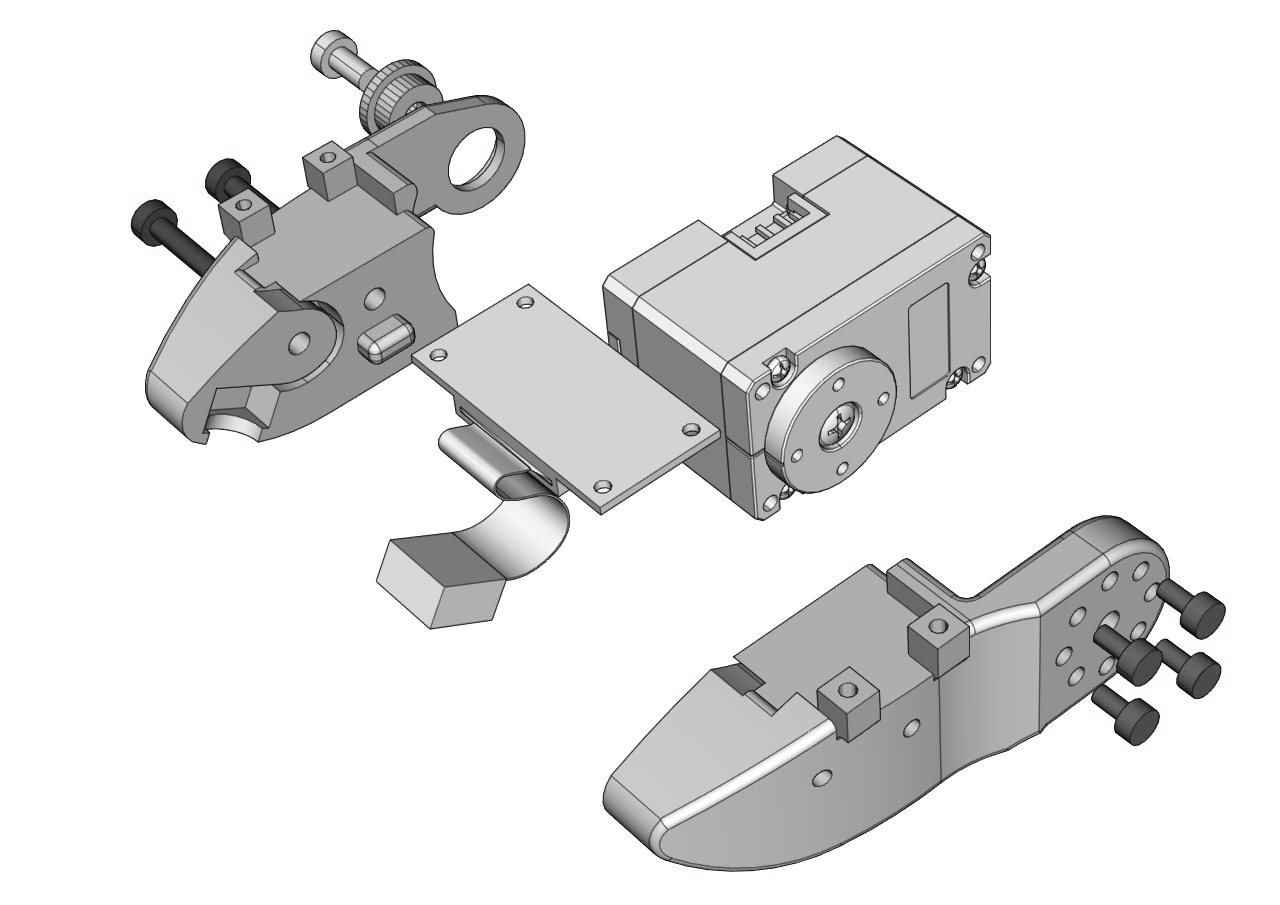
\includegraphics[width=\linewidth]{figures/finger_exploded_gray.png}
\par\vspace{3mm}Exploded View
\end{minipage}\hfill
\begin{minipage}[t]{.49\textwidth}
\vspace{0pt}\centering
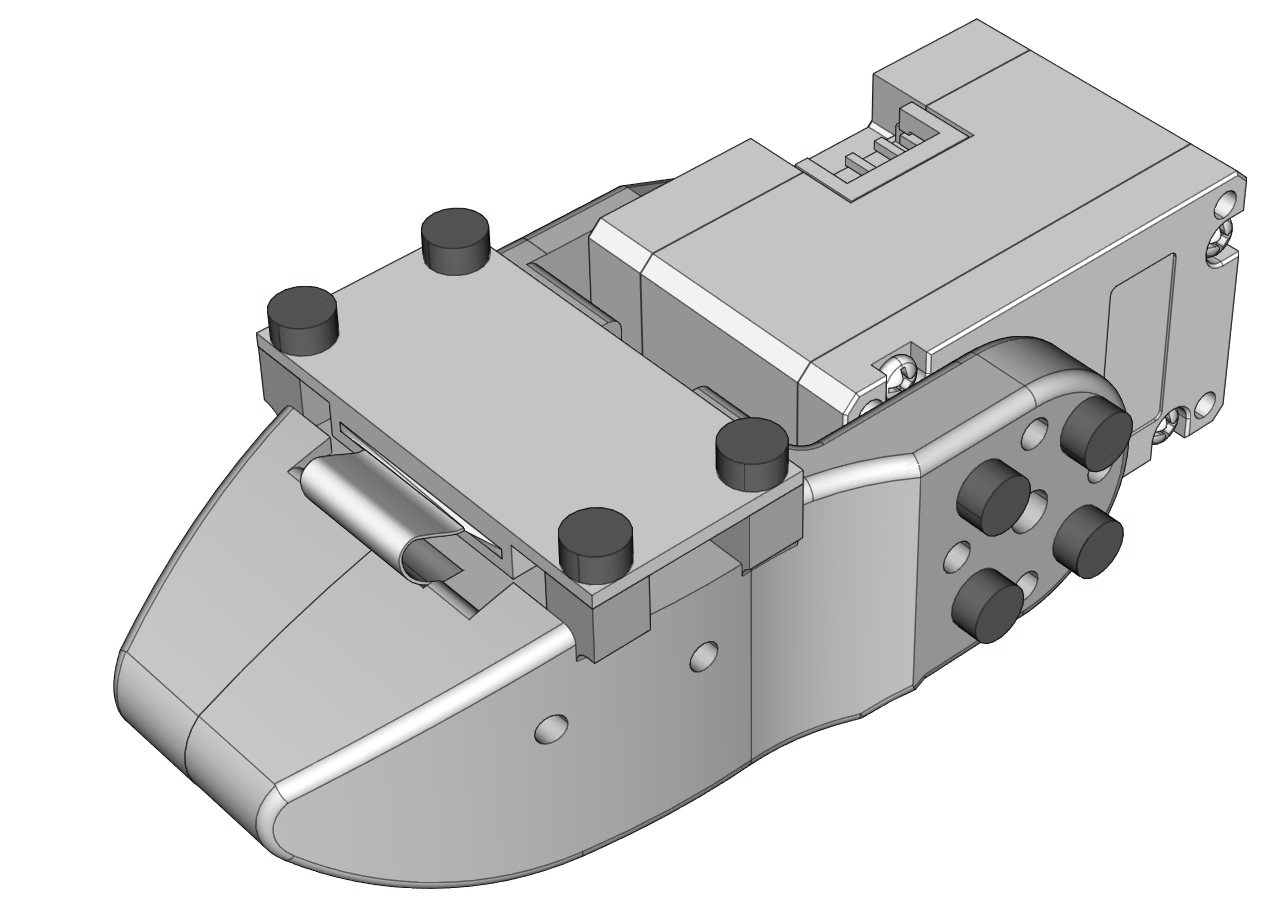
\includegraphics[width=\linewidth]{figures/finger_closed_gray.png}
\par\vspace{3mm}Assembled View
\end{minipage}
\end{document}
